\documentclass[letterpaper, 10 pt, conference]{ieeeconf}  % Comment this line out if you need a4paper
\usepackage{graphicx} % Required for inserting images
\usepackage{amsmath}
\usepackage{hyperref}
\usepackage{float}
\usepackage{biblatex}
\usepackage{tikz}
\usepackage{gensymb}
\usetikzlibrary{arrows.meta, positioning}

\hypersetup{
	colorlinks=true,       % false: boxed links; true: colored links
	linkcolor=blue,        % color of internal links
	citecolor=blue,        % color of links to bibliography
	filecolor=magenta,     % color of file links
	urlcolor=blue         
}

\bibliography{refs}

\title{\LARGE \bf Model-Based Fixed Wing Swarms}
\author{Archit Swamy, Leena Vacchani, Shashiranjan Kumar}% <-this % stops a space
\thanks{*This work was supported by XYZ}% <-this % stops a space
\thanks{Archit Swamy is with the Department of Electrical Engineering, University of XYZ, City, Country
        {\tt\small archit.swamy@xyz.edu}}%


\begin{document}

\maketitle
\thispagestyle{empty}
\pagestyle{empty}

\begin{abstract}
In this paper, we present a new algorithm designed to facilitate coordinated flocking behavior among fixed-wing unmanned aerial vehicles (UAVs) in two-dimensional environments. Unlike traditional flocking algorithms primarily developed for rotary-wing or ground-based agents, our approach specifically addresses the kinematic constraints of fixed-wing flight using a toy model. The algorithm ensures collision avoidance and maintains cohesive group movement, allowing for scalable operations in various 2D scenarios. 
\end{abstract}

\section{Introduction}

The development and deployment of unmanned aerial vehicles (UAVs) have seen significant advancements in recent years, leading to a wide range of applications in both military and civilian domains. Among these applications, the concept of UAV swarms has garnered particular interest due to their potential for enhanced efficiency, robustness, and scalability in performing complex tasks. While much of the existing research on UAV swarms has focused on rotary-wing or ground-based vehicles, fixed-wing UAVs present unique challenges and opportunities due to their distinct kinematic constraints and flight dynamics.

This paper introduces a novel algorithm designed to enable coordinated flocking behavior among fixed-wing UAVs operating in two-dimensional environments. Traditional flocking algorithms, such as those based on Olfati-Saber's framework, typically assume agents with unconstrained maneuverability, making them less suitable for fixed-wing UAVs that must adhere to minimum velocity requirements and specific turning radii. Our approach addresses these limitations by incorporating a toy model that captures the essential dynamics of fixed-wing flight.

The proposed algorithm ensures collision avoidance and cohesive group movement, leveraging concepts from graph theory and control theory to manage the interactions and movements of the UAVs. By maintaining a balance between local interactions and global objectives, the algorithm allows for scalable and efficient operations in various 2D scenarios. The introduction of actuator saturation constraints and modifications to traditional consensus terms further enhance the algorithm's applicability to fixed-wing UAVs.

This work contributes to the growing body of knowledge on UAV swarms by providing a tailored solution for fixed-wing platforms, addressing key challenges such as collision avoidance, heading alignment, and speed matching. The results demonstrate the feasibility of achieving stable and cohesive flocking behavior, paving the way for more advanced and reliable swarm-based missions involving fixed-wing UAVs.

\section{Preliminaries}

\subsection{Olfati-Saber Flocking}

\subsubsection{Reynold's Rules}

\noindent Olfati-Saber flocking was developed to model point objects with no constraints on maneuverability. As such, the follow Reynold's rules of flocking, consisting of three heuristics:
\begin{itemize}
    \item Flock Centering: attempt to stay close to nearby flockmates
    \item Collision Avoidance: avoid collisions with nearby flockmates
    \item Velocity Matching: attempt to match velocity with nearby flockmates
\end{itemize}

\subsubsection{Relevant Graph Theory}

For the purpose of flocking, we will work with graphs that depict spatial information. A graph $G$ is a pair $(V,E)$ that consists of vertices $V = \{1,2...,n\}$ and edges $E \subseteq \{(i,j) : i,j \in V, j \neq i\}$. The adjacency matrix, denoted as \(A\), is a square matrix representing the connections or interactions between individual agents in the swarm. It is often used to describe the topology or network structure of the swarm. Each entry \(A_{ij}\) of the adjacency matrix is defined as follows:

\[
A_{ij} =
\begin{cases}
    1 & \text{if } (i,j) \in E \\
    0 & \text{otherwise } 
\end{cases}
\]

Adjacency matrices can be used as weighted graphs by replacing the 0,1 elements with varying weights. For an undirected graph $G$, the adjacency matrix is symmetric i.e, $A^T = A$. Using the adjacency matrix, we can define the in-degree, out-degree and neighbour set of the $i^{th}$ agent. The row sum $(\sum_{j=1}^N a_{ij})$ indicates the out-degree of the $i^{th}$ agent, the column sum $(\sum_{j=1}^N a_{ji})$ indicates the in-degree, and the neighbour set is defined as follows: 

\begin{equation}
    N_i = \{j \in V:a_{ij} \neq 0 \} = \{j \in V:(i,j) \in E \}
\end{equation}

The Laplacian matrix, denoted as \(L\), is derived from the adjacency matrix and is a key component in analyzing the collective behavior of a swarm. It is defined as:

\[
L = D - A
\]

where \(D\) is the degree matrix, a diagonal matrix where \(D_{ii}\) represents the degree of agent \(i\), i.e., the number of connections or interactions it has. The Laplacian matrix \(L\) captures the relationship between an agent and its neighbors, and it plays a crucial role in characterizing the dynamics of the swarm.

% In swarm algorithms, the eigenvalues and eigenvectors of the Laplacian matrix are used to study stability, connectivity, and synchronization properties of the swarm, which are essential for understanding the emergent behavior of the group of agents.

% These matrices are foundational in the mathematical analysis of swarm algorithms, allowing for the investigation of how the local interactions among agents give rise to global swarm behaviors.

Let $q_i, p_i \in \mathcal{R}^m$ denote the position and velocity of the $i^{th}$ agent. Thus the dynamics of the system are given as 

\[
\begin{cases}
  \dot{q_i} = p_i \\
  \dot{p_i} = u_i
\end{cases}
\]

where $u_i$ is the control input, or the acceleration applied to the agent. 

Now we bake the distributed nature of the network into the equations using the neighbour set $N_i$. We define an interaction range $r$ between two agents. 

\begin{equation}
    N_i = \{j \in V:||q_j-q_i||<r\}
\end{equation}

where $||\cdot||$ is the Euclidean norm in $R^m$. Thus we are able to define our adjacency matrix in a similar manner. 

\begin{equation}
    A_{ij} = 
    \begin{cases}
        1, & \text{if } ||q_j-q_i|| < r \\
        0, & \text{otherwise}
    \end{cases}
\end{equation}

\textbf{Definition\cite{1605401}:} $\alpha$-lattices are structures in which all neighbouring agents are at a distance $d$ from each other. The scale and ratio of the graph are defined as $d$ and $\kappa = r/d$. 

\begin{equation}
    ||q_j-q_i|| = d \ \forall \ j \in N_i(q)
\end{equation}

As a measurement of the deviation of a given flock structure from an alpha lattice, we define a deviation energy

\begin{equation}
    E_{\delta}(q) = \frac{1}{|E|+1}\sum_{i=1}^N\sum_{j\in N_i}\psi (||q_j-q_i|| - d)
\end{equation}

For a quasi-$\alpha$-lattice, with $|||q_j-q_i|| - d| < \delta$, we get that the deviation energy is bounded

\begin{equation}
    E_\delta(q) \leq \frac{|E(q)|}{|E(q)|+1} \delta^2 \leq \delta^2 = \epsilon^2d^2, \ \ \epsilon << 1
\end{equation}

Thus, we see that the alpha lattices are low-energy configurations of the $N$ agents. The work herein tries to mimic, and recreate these alpha lattices for 2D fixed-wing agents constrained in curvature. In doing so, we will find that the deviation energy serves as a useful metric. 

\subsubsection{Smooth Collective Potentials}

As in \cite{1605401}, a smooth potential function $(\psi_\alpha)$ is defined: 

\begin{align}
    ||z||_\sigma = & \ \frac{1}{\epsilon}(\sqrt{1 + \epsilon||z||^2} - 1) \\
    \sigma_\epsilon(z) = & \ \frac{z}{\sqrt{1 + \epsilon||z||^2}} \\
    \rho_h(z) = & \ 
    \begin{cases}
        1, & z \in [0,h) \\
        \frac{1}{2}[1 + cos(\pi\frac{z-h}{1-h})], & z \in [h,1] \\
        0, & \text{otherwise}
    \end{cases} \\
    \phi(z) = & \ \ \frac{1}{2}[(a+b)\sigma_1(z+c) + (a-b)] \\
    \phi_\alpha(z) = & \ \ \rho_h(z/r_\alpha)\phi(z-d_\alpha) \\
    \psi_\alpha(z) = & \ \int_{d_\alpha}^z \phi_\alpha(s) ds
\end{align}

This results in the following force $(\phi_\alpha)$ profile:

\begin{figure}[H]
    \centering
    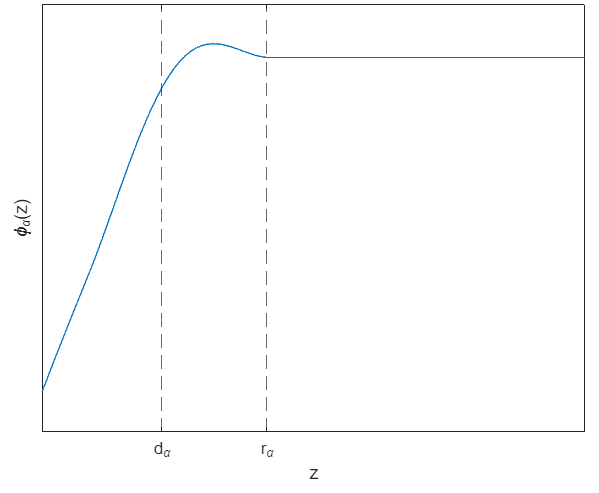
\includegraphics[width=0.75\linewidth]{imgs/phialpha.png}
    \caption{$\phi_\alpha(z)$}
    \label{fig:enter-label}
\end{figure}

The force acting on the agent is given by the derivative of this potential function, namely $\phi_\alpha(z)$.

Using this potential function $\psi_\alpha$, we define an energy associated with the set of agents based on their positions $\mathbf{q}$. 

\begin{equation}
    V(\mathbf{q}) = \frac{1}{2}\sum_{i=1}^N \sum_{j \neq i} \psi_\alpha(||q_j-q_i||_\sigma)
\end{equation}

\subsection{Drawbacks of Olfati}

Olfati fails in many aspects when being applied to real-world systems for the purpose of control.

\begin{itemize}
    \item The inter-agent potentials are, in a sense, heading-independent. Forces can be applied to agents in arbitrary directions, which is why the flocking law so easily generalises to $n$-dimensions. This clearly fails when constraints are introduced, such as the dynamics of fixed-wings. 
    \item Flocking is performed in a completely distributed sense, with respect to a given sensing radius which must be kept finite. This implies the graph describing inter-agent sensing may not be connected at some time $t$. This leads to sub-flocks that do not interact with each other. 
    \item Olfati fails spectacularly with the fixed-wing model. This can be understood quite simply by noting that two agents in a head-on collision tend only to decelerate under the Olfati law, in an attempt to turn through a zero velocity. Fixed-wings, however, need to maintain some minimum velocity and must therefore turn as much as possible to avoid a collision.
\end{itemize}

\subsection{Fixed Wing Model}

Fixed wing aircraft (in 2D) can be assumed to move as cars on banked roads, where one can control the bank angle. Fixed wings are also constrained such that they must, at all times, have a non-zero velocity $v_{min}$. Specifically,

\begin{center}
\begin{align}
v_{min} < v & < v_{max}\\
R \ =  \ & \frac{v^2}{g\tan\phi}\\
-\phi_{max} < \phi & < \phi_{max}
\end{align}
\end{center}

where $R$ is the turning radius, and $\phi$ is the bank (roll) angle. These bounds are maintained manually within the algorithm; if the velocity is at the bounds, we multiply the acceleration applied to the agents with a step function. 

Let $u(x_0)$ denote a step function, 

\begin{equation}
    u(x_0) = 
    \begin{cases}
        0, x < x_0 \\
        1, x \geq x_0
    \end{cases}
\end{equation}

Thus, algorithmically, the acceleration applied to an agent is determined as,

\begin{equation}
    a = 
    \begin{cases}
        a * u(0), \ \ \ \ \ \ \ \ v = v_{min} \\
        a, \ \ \ \ \ \ \ \ \ \ \ \ \ \ \ \ v_{min} < v < v_{max} \\
        a  * (1 - u(0)), \ v = v_{max}
    \end{cases}
\end{equation}

\section{Forming Flocks}

Noting the challenges with Olfati mentioned above, I propose modifications to the flocking law so that it fits the fixed-wing model and a planning approach to flocking which ensures the formation of one single cohesive flock (this requires global communication).

\subsection{Replacing the Consensus term}

The consensus term within the Olfati framework was simple yet effective; it accounted for two effects: alignment and damping.

\begin{equation}
    \dot{\mathbf{p}}_i = \sum_j a_{ij}(\mathbf{p}_j - \mathbf{p}_i)
\end{equation}

In order to accommodate the fixed-wing model, we replace this part of the flocking law with two heuristic laws, one for each of the effects of the consensus term. The total consensus term may then be represented as,

\begin{equation}
    \dot{\mathbf{p}}_i = \boldsymbol{\omega}_i \times \mathbf{p}_i + f_i^d \hat{\mathbf{p}}_i
\end{equation}

where $\boldsymbol{\omega}_i$ is $\omega_i\hat{\mathbf{z}}$. 

\vspace{5pt}

\subsubsection{Alignment}
(Note that all angles are measured w.r.t a fixed coordinate frame) This force causes the agent to turn toward a target heading. Assuming some target heading $\theta_T$, the turning force is given as,

\begin{equation}
    \omega_i = \dot{\theta}_i = -A\frac{\eta_i}{||\mathbf{p}_i||}
\end{equation}

where $\eta_i$ is the deviation of the $i^{th}$ agent's heading and the target heading. In particular, it can be given by the form,

\begin{equation}
    \eta_i = \min(\theta_i - \theta_T, 2\pi - (\theta_i - \theta_T))
\end{equation}

\begin{equation}
    \dot{\eta}_i = \min(\dot{\theta}_i, -\dot{\theta}_i)
\end{equation}

Thus, we have the well-known form which is globally exponentially stable in error,

\begin{equation}
    \dot{\eta}_i = -A\frac{\eta_i}{||\mathbf{p}_i||}
\end{equation}

This guarantees convergence in heading. 

\vspace{5pt}

\subsubsection{Damping}
In actuality, this term serves to match the speeds of different agents, rather than simply damping energy out of the system. This term is based on the following heuristics:

\begin{itemize}
    \item If the relative velocity of two agents is aligned perpendicularly to their respective velocities, then they should feel no need to speed up or slow down. 
    \item If the relative velocities of two agents is parallel to an agent's velocity, it should speed up as the other agent in question is moving faster.
    \item If the relative velocities of two agents is anti-parallel to an agent's velocity, it should slow down as the other agent in question is moving slower/towards the agent.
\end{itemize}

The particular form of the damping term is as follows,

\begin{equation}
    f_i^d = \sum_{j \in \mathcal{N}_i}a_{ij}((\mathbf{p}_j - \mathbf{p}_i)\cdot\frac{\mathbf{p}_i}{||\mathbf{p}_i||}) 
\end{equation}

\begin{equation}
    f_i^d = \sum_{j \in \mathcal{N}_i} a_{ij}(||\mathbf{p}_j||cos\gamma_{ij} - ||\mathbf{p}_i||)
\end{equation}

where $\mathcal{N}_i$ is the neighbour set of agent $i$, $\gamma_{ij}$ is the angle between agent $i$'s and $j$'s headings. This can be understood as the difference between agent $j$'s and agent $i$'s speeds along $i$'s heading, scaled by a directional term, $cos\gamma$. It is also clear that this force term can also be made to fit the actuator saturation method above as it is upper bounded by $2v_{max}$. 

This results in a final flocking law:

\begin{equation}
        \dot{\mathbf{p}}_i = \mathbf{f}_i^g + \boldsymbol{\omega}_i\times\mathbf{p}_i + f_i^d \hat{\mathbf{p}}_i
\end{equation}

where $\mathbf{f}_i^g$ is the Olfati force, given by $-\nabla V(\mathbf{q})$.

\subsection{Actuator Saturation}

Given the toy model of fixed wings we have considered, we can make a simplifying assumption: the forces exerted by the actuators on the agent are saturated independently in the directions parallel $(F^{||}_{max})$ and perpendicular to the agent's heading $(F^{\perp}_{max})$. This assumption holds as long as the maximum bank angle $\phi_{max}$ is small. 

The new consensus terms, alignment and damping, are both individually saturated. Olfati's smooth collective potential, due to the weighting applied by the adjacency matrix $\{a_{ij}\}$, is also saturated. Therefore, there are three forces acting on any given agent. 

In dealing with actuator saturation then, we need only consider two cases: the olfati force on the agent is a) parallel to the acceleration and b) parallel to the turning force.  

\begin{figure}[H]
\centering
\begin{tikzpicture}

% First diagram
\node[inner sep=0pt] (case1) at (0,0) {
  \begin{tikzpicture}
    % Agent (scaled up 3 times from previous 10 times smaller)
    \fill (0,0) -- (0.3,0) -- (-0.1,0.15) -- cycle;
    \fill (0,0) -- (0.3,0) -- (-0.1,-0.15) -- cycle;
    % Olfati force
    \draw[->, thick, red] (0.15,0) -- (1.15,0) node[right, red, above=5pt] {Olfati};
    % Heading (turning) force
    \draw[->, thick, dashed] (0.15,0) -- (0.15,0.85) node[above] {Heading};
    % Damping force
    \draw[->, thick, dashed] (0.15,0) -- (1,0) node[right, below=5pt] {Damping};
  \end{tikzpicture}
};

% Second diagram
\node[inner sep=0pt, right=1cm of case1] (case2) {
  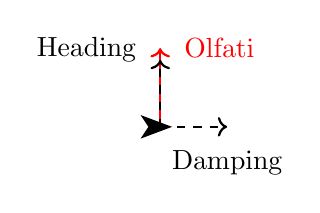
\begin{tikzpicture}
    % Agent (scaled up 3 times from previous 10 times smaller)
    \fill (0,0) -- (0.3,0) -- (-0.1,0.15) -- cycle;
    \fill (0,0) -- (0.3,0) -- (-0.1,-0.15) -- cycle;
    % Olfati force
    \draw[->, thick, red] (0.15,0) -- (0.15,1) node[right, right=5pt, red] {Olfati};
    % Heading (turning) force
    \draw[->, thick, dashed] (0.15,0) -- (0.15,0.85) node[left, xshift=-5pt, pos=1.16] {Heading};
    % Damping force
    \draw[->, thick, dashed] (0.15,0) -- (1,0) node[right, below=5pt] {Damping};
  \end{tikzpicture}
};

\end{tikzpicture}
\caption{Two Bounding Cases on Actuator Saturation} \label{fig:M1}
\end{figure}

Let us notate the forces as the following: $O$ (Olfati), $H$ (Heading), $D$ (Damping). Recalling the constraints imposed on the actuators, and from the two diagrams above, for actuator saturation to hold, we require the following conditions to hold:

\begin{align}
    O_{max} + H_{max} \leq F^{\perp}_{max}\\
    O_{max} + D_{max} \leq F^{||}_{max}
\end{align}

These two conditions imply that the controller must be tuned based on model parameters. This will then ensure that actuator saturation is maintained. 

\subsection{Collision Avoidance}

In order to deal with collisions, we try to simplify the problem slightly. Trying to avoid collisions given any initial random state is a hard problem to tackle. Not to mention, it is obviously impossible in some cases, and to find constraints on starting conditions which would ensure no collisions is a problem that scales with the number of agents and the complexity of the flocking law, and is therefore infeasible (within my work as an undergraduate).

Therefore, we introduce a "planning" step in the flocking scheme, where all the agents align themselves. Thus, all these agents form aligned subflocks which can merge with each other. Further collision avoidance is handled by the Olfati law. 

\begin{figure}[H]
    \centering
    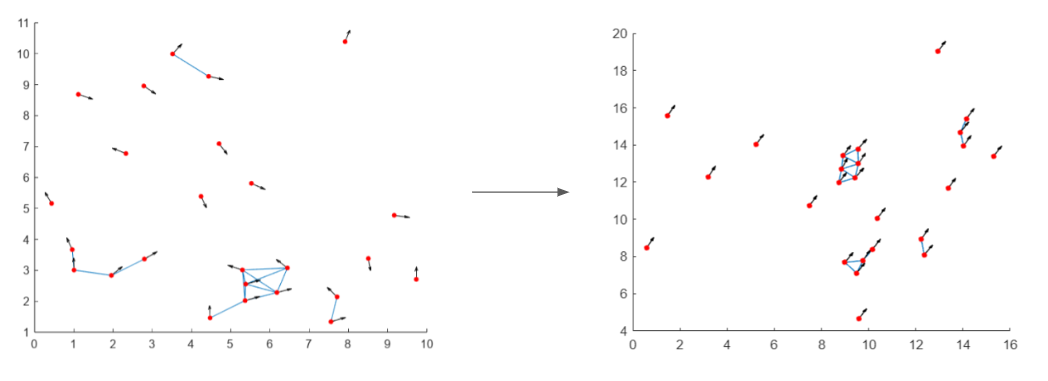
\includegraphics[width=\linewidth]{imgs/alignment.png}
    \caption{Alignment Scheme}
    \label{fig:alignment}
\end{figure}

However, it is important to avoid collisions even during the alignment step. The simplest solution to this is to start off with only those initial conditions where the minimum inter-agent distance is some $D_{min}$. During this alignment step, we should note that the agents are considered to move in a free space (no obstacles) and are only concerned with aligning themselves to a global target heading. 

In order to determine a value on $D_{min}$, we can use a heuristic based on Dubin's path \cite{aac5c909-7434-3d95-961b-caf3aec6a743}. Assuming the worst case scenario, where the radius of curvature of the agent's path is maximum due to the agent having maximum velocity, assuming maximum turning, we get a radius,

\begin{equation}
    R_{max} = \frac{v_{max}^2}{g\tan\phi_{max}}
\end{equation}

In the worst case scenario, we would have two agents at the opposite ends of two diameters joined together, turning in the same direction, as shown below. 

\begin{figure}[H]
\centering
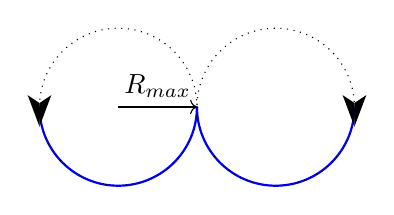
\begin{tikzpicture}
    % Draw the radius
    \draw[->] (-1,0) -- (0,0) node[midway, above] {$R_{max}$};

    % Draw the blue semicircles
    \draw[blue, thick] (0,0) arc[start angle=0, end angle=-180, radius=1cm];
    \draw[blue, thick] (0,0) arc[start angle=-180, end angle=0, radius=1cm];

    % Draw the black dotted circles
    \draw[black, dotted] (0,0) arc[start angle=180, end angle=540, radius=1cm];
    \draw[black, dotted] (0,0) arc[start angle=0, end angle=360, radius=1cm];

    % Draw the agents
    \fill (-2,0.05) -- (-2,-0.25) -- (-2.15,0.15) -- cycle;
    \fill (-2,0.05) -- (-2,-0.25) -- (-1.85,0.15) -- cycle;
    \fill (2,0.05) -- (2,-0.25) -- (2.15,0.15) -- cycle;
    \fill (2,0.05) -- (2,-0.25) -- (1.85,0.15) -- cycle;
\end{tikzpicture}
\caption{Worst Case during Alignment Step}
\end{figure}

Thus our heuristic evaluates to $D_{min} = 4R_{max}$.

Let us test this heuristic in simulation. We can assume, during the alignment step, that each agent is only concerned with aligning itself to some common target heading and does not change its speed. The turning term introduced as part of the replacement to Olfati's flocking law serves this exact purpose. 

Here we perform a monte carlo simulation for each value of $D_{min}$, where $D_{min}$ is the minimum distance between any two agents at $t=0$. For each $D_{min}$, we perform 100 simulations in order to estimate an average number of collisions. In each run, all agents are initialized at random positions, maintaining a minimum inter-agent distance of $D_{min}$, with randomized velocities. To ensure that we obtain a lower bound on $D_{min}$, we initialize the agents uniformly within the smallest square region which satisfies the minimum inter-agent distance constraint. Specifically, if $D_{min}$ is set to $a$, and there are $n^2$ agents, the agents are initalised as shown below, with randomised velocities.

\begin{figure}[H]
    \centering
    \begin{tikzpicture}
        \def\n{5}  % number of dots per line
        \def\a{0.6}  % distance between dots
        
        % Draw the grid of dots
        \foreach [count=\i] in {0, 1, ..., \n-1} {
            \foreach [count=\j] in {0, 1, ..., \n-1} {
                \fill (\i*\a, \j*\a) circle (2pt);
            }
        }
        
        % Draw the line and label for distance a
        \draw[<->] (0.05, 0) -- (\a-0.05, 0) node[midway, above] {$a$};
    \end{tikzpicture}
    \caption{Initialised Positions on Collision Testing}
    \label{fig:enter-label}
\end{figure}

Simulation parameters: 

$$v_{max} = 2, g = 1, \phi_{max} = 45 \degree$$

\begin{figure}[H]
    \centering
    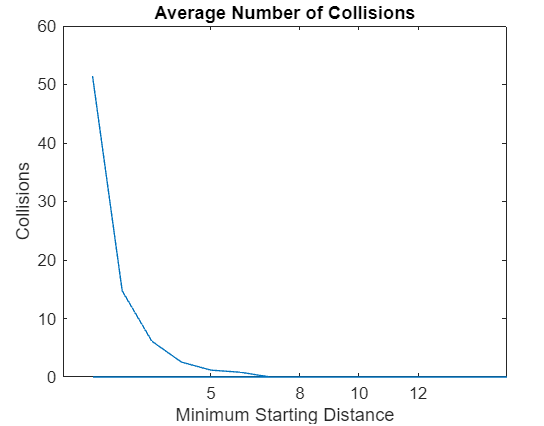
\includegraphics[width=0.75\linewidth]{imgs/collisions_vs_initial_distance.png}
    \caption{Collisions versus Minimum Starting Distance}
    \label{fig:enter-label}
\end{figure}

\subsection{Merging Subflocks}

This is the crucial step in flock formation. This modification to Olfati's law makes it so that the flock does not suffer from the major problem of being disconnected fragments. 

In order to merge fragments, we propose a scalable solution: treat an entire fragment as one agent, in a system where the sensing radius $r$ and the alpha lattice parameter $d$ are set to values such that their ratio $\kappa$ remains constant, and the nearest unconnected fragment is at some distance between $x > r$. The protocol simply updates $d$ and $r$ over time, so that the fragments experience an attractive force, essentially annealing the parameters so that $r \rightarrow r_0$. This modified $(d, r)$ Olfati force is applied to all the agents in the fragment.  

If we look at the profile of the potential function $\psi_\alpha$, the agents (and hence fragments) will experience an attractive force whilst $d < x < r$. Additionally, the slope (and hence the force) is greatest near the middle $x = \frac{d + r}{2}$. Hence, we arrive at the simplest protocol to merge fragments. Given $\kappa = \frac{r}{d}$, we set $d, r$.

\begin{align}
    d = & \ \frac{2x}{\kappa+1} \\
    r = & \ \kappa d
\end{align}

Over time, the fragments coalesce as they brought closer to one another. If during this step, a third fragment approaches one of the two fragments such that it is now the closest fragment to one of the original two fragments, the switching behaviour is not an issue as the values $d, r$ vary smoothly based on the distance of the nearest fragment, which must be equal at the time of the switching. 

\subsection{Stability Analysis}

Since we apply the same flocking law at both, the agent level and the fragment level, showing that the system is stable (forms flocks) implies that fragments are formed at the agent level, and fragments coalesce at the fragment level. 

Given a total energy hamiltonian,

\begin{equation}
    H(\mathbf{q}, \mathbf{p}) = V(\mathbf{q}) + \frac{1}{2}\mathbf{p}^T\mathbf{p} 
\end{equation}

\begin{equation}
    \dot{H} = \nabla V(\mathbf{q}) \dot{\mathbf{q}} + \mathbf{p}^T\dot{\mathbf{p}}
\end{equation}

Expanding $\dot{\mathbf{p}}$, we have,

\begin{equation}
    \dot{H} = \nabla V(\mathbf{q}) \dot{\mathbf{q}} + \mathbf{p}^T\{ -\nabla V(\mathbf{q}) + \boldsymbol{\omega}\times\hat{\mathbf{p}} + f^d \hat{\mathbf{p}} \}
\end{equation}

\begin{equation}
    \dot{H} = \sum_{i=1}^n \{[\mathbf{p}_i \ \boldsymbol{\omega}_i \ \mathbf{p}_i] + f_i^d \mathbf{p}_i \cdot \hat{\mathbf{p}}_i\}
\end{equation}

\begin{equation}
    \dot{H} = \sum_{i=1}^n f_i^d ||\mathbf{p}_i|| 
\end{equation}

\begin{equation}
    \dot{H} = \sum_{i=1}^n \{ \sum_{j \in \mathcal{N}_i} a_{ij}(||\mathbf{p}_j||cos\gamma_{ij} - ||\mathbf{p}_i||) \} ||\mathbf{p}_i||
\end{equation}

\begin{equation}
    \dot{H} = \sum_{i, j} a_{ij} (||\mathbf{p}_i|| \cdot ||\mathbf{p}_j|| \cos\gamma_{ij} - ||\mathbf{p}_i||^2) 
\end{equation}

where we have switched the limits for the summation of $j$ from $j \in \mathcal{N}_i$ to $j \in \{1, \cdots, n\}$. These are equivalent as $a_{ij} = 0$ if $j \notin \mathcal{N}_i$. Note that $a_{ii}$ is also equal to $0$ for all $i$.

\begin{equation}
    \dot{H} = \frac{1}{2} \sum_{i,j} (2 ||\mathbf{p}_i|| \cdot ||\mathbf{p}_j|| \cos\gamma_{ij} - ||\mathbf{p}_i||^2 - ||\mathbf{p}_j||^2)
\end{equation}

\begin{equation}
    \dot{H} = -\frac{1}{2} \sum_{i,j} (\mathbf{p}_i - \mathbf{p}_j) \cdot (\mathbf{p}_i - \mathbf{p}_j)
\end{equation}

\begin{equation}
    \dot{H} = -\frac{1}{2} \sum_{i,j} ||\mathbf{p}_i - \mathbf{p}_j||^2
\end{equation}

Thus, $H$ is Lyapunov stable. The agents will, in time, form one cohesive flock where the distance between any two neighbouring agents is $d$.

\section{Results in Simulation}

\subsection{Simulator Validation}



\subsection{Flocking Results}

\subsection{Boundedness of Control Inputs}

\section{Further Scope}

\section{Acknowledgement}

The authors would like to thank Rohan Waghmare, Anushka Sinha, and Aakash Chaphalkar of L\&T Defense for funding this research.

\printbibliography

\end{document}
